\documentclass[tikz,dvisvgm,border=10pt]{standalone}
\usetikzlibrary{shapes.geometric,shapes.symbols,shapes.callouts,shapes.multipart,shapes.misc,arrows,positioning,fit,backgrounds,shadows}

\begin{document}
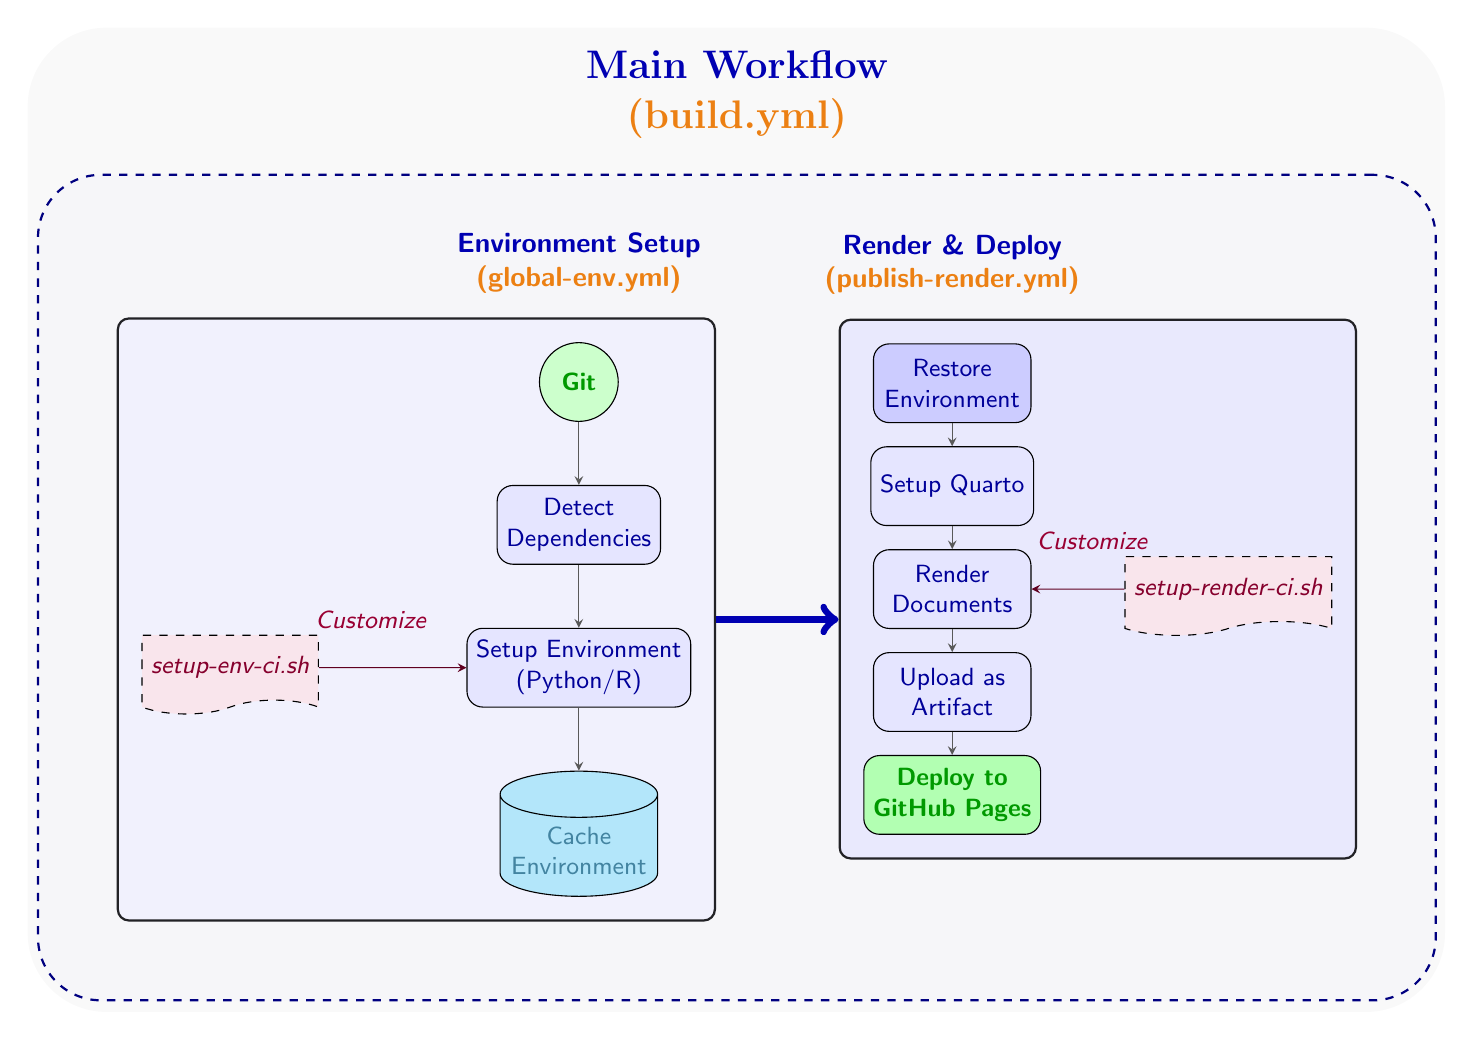
\begin{tikzpicture}[
    % Define styles for nodes with enhanced colors
    doc/.style={draw, minimum width=5cm, minimum height=2cm, align=center, fill=blue!20, text=blue!80!black, font=\bfseries, rounded corners=3mm, drop shadow},
    container/.style={draw=blue!50!black, fill=blue!10, fill opacity=0.15, inner sep=10mm, rounded corners=8mm, thick, dashed},
    package/.style={draw, fill=blue!5, fill opacity=0.7, inner sep=3mm, rounded corners, text=blue!60!black, thick},
    process/.style={draw, minimum width=2cm, minimum height=1cm, align=center, fill=blue!10, text=blue!60!black, font=\small\sffamily, rounded corners=2mm},
    cylnode/.style={draw, cylinder, shape border rotate=90, aspect=0.3, minimum height=1cm, minimum width=2cm, align=center, fill=cyan!30, text=cyan!60!black, font=\small\sffamily},
    dashboard/.style={circle, draw, minimum size=1cm, fill=green!20, text=green!60!black, font=\small\sffamily\bfseries},
    document/.style={draw, shape=tape, tape bend top=none, minimum width=2cm, minimum height=1cm, align=center, dashed, fill=purple!10, text=purple!70!black, font=\small\sffamily\itshape},
    thick_arrow/.style={->, line width=1mm, draw=blue!70!black},
    arrow/.style={->, >=stealth, draw=gray!70!black},
    title/.style={font=\bfseries\sffamily, align=center, text width=4cm, text=blue!70!black},
    label/.style={font=\small\sffamily\itshape, inner sep=2pt, text=purple!80!black},
    filename/.style={font=\small\sffamily\itshape, text=orange!70!brown}
]

% Add a background for the entire diagram
\begin{scope}[on background layer]
    \fill[rounded corners=10mm, gray!5] (-2,-8) rectangle (16,4.5);
\end{scope}

% Create environment steps first
\node[dashboard] (checkout) at (5,0) {Git};
\node[process, below=0.8cm of checkout] (detect) {Detect\\Dependencies};
\node[process, below=0.8cm of detect] (setup) {Setup Environment\\(Python/R)};
\node[cylnode, below=0.8cm of setup] (cache) {Cache\\Environment};

% Environment connections
\draw[arrow] (checkout) -- (detect);
\draw[arrow] (detect) -- (setup);
\draw[arrow] (setup) -- (cache);

% Custom environment script - with label higher
\node[document] (customenv) at ([xshift=-3cm]setup.west) {setup-env-ci.sh};
\draw[arrow, draw=purple!50!black] (customenv) -- (setup) node[pos=0.35, above=12pt, label] {Customize};

% Environment setup container with title above
\node[title] at (checkout.north) [above=5mm] {Environment Setup \\\textcolor{orange!70!brown}{(global-env.yml)}};

% Use layers to put containers in the background - adjusted fit
\begin{scope}[on background layer]
    \node[package, fill=blue!5] (env) [fit=(checkout) (detect) (setup) (cache) (customenv)] {};
\end{scope}

% Create render steps first - explicitly aligned with env.east anchor
\path (env.east) ++(3cm,0) coordinate (render_start);
\node[process, fill=blue!20] (restore) at ([yshift=3cm]render_start) {Restore\\Environment};
\node[process] (quarto) at ([yshift=-0.8cm]restore.south) {Setup Quarto};
\node[process] (compile) at ([yshift=-0.8cm]quarto.south) {Render\\Documents};
\node[process] (artifact) at ([yshift=-0.8cm]compile.south) {Upload as\\Artifact};
\node[process, fill=green!30, text=green!60!black, font=\small\sffamily\bfseries] (deploy) at ([yshift=-0.8cm]artifact.south) {Deploy to\\GitHub Pages};

% Render connections
\draw[arrow] (restore) -- (quarto);
\draw[arrow] (quarto) -- (compile);
\draw[arrow] (compile) -- (artifact);
\draw[arrow] (artifact) -- (deploy);

% Custom render script - with label higher and inverted direction
\node[document] (customrender) at ([xshift=2.5cm]compile.east) {setup-render-ci.sh};
\draw[arrow, draw=purple!50!black] (customrender) -- (compile) node[pos=0.35, above=12pt, label] {Customize};

% Render and deploy container with title above
\node[title] at (restore.north) [above=5mm] {Render \& Deploy \\\textcolor{orange!70!brown}{(publish-render.yml)}};

% Use layers to put containers in the background - adjusted fit
\begin{scope}[on background layer]
    \node[package, fill=blue!10] (render) [fit=(restore) (quarto) (compile) (artifact) (deploy) (customrender)] {};
\end{scope}

% Main flow connections
\draw[thick_arrow] (env.east) -- (render.west |- env.east);

% Finally create the main workflow container around everything
\begin{scope}[on background layer]
    % Create invisible nodes to capture the title areas
    \node[opacity=0] (env_title_anchor) at ([yshift=10mm]checkout.north) {};
    \node[opacity=0] (render_title_anchor) at ([yshift=10mm]restore.north) {};
    
    % Make container fit these invisible nodes too, ensuring it goes high enough
    \node[container, fit=(env_title_anchor) (render_title_anchor) (env) (render)] (workflow_container) {};
    
    % Place the title well above the container with colored filename
    \node[font=\bfseries\Large, text=blue!70!black, align=center] at ([yshift=10mm]workflow_container.north) {Main Workflow \\\textcolor{orange!70!brown}{(build.yml)}};
\end{scope}

\end{tikzpicture}
\end{document}